\documentclass{beamer}
\usepackage{ngerman}
\usepackage[utf8]{inputenc}
\usepackage{amsmath,amsfonts,amssymb}
\usepackage{graphicx}
\usepackage{multirow}
\usepackage{listings}
\usepackage{hyperref}
\usepackage{tikz}
\usetikzlibrary{automata}
\usetheme{HUmetrics}
\usecolortheme{default}
\usefonttheme{serif}
%\useinnertheme{circles}
\setbeamertemplate{navigation symbols}{}
\lstset{language=[LaTeX]TeX,
	basicstyle=\tiny,
	stringstyle=\ttfamily,
	commentstyle=,
	tabsize=2,
	numbers=left,
	frame=single,
	framerule=0.1pt,
	keywordstyle=\color{blue}
}

\title[MOJITO]{Measurements and Optimizations with Just-In-Time code generation on the OpenFlow reference implementation}
\author[Samuel Brack]{Samuel Brack}
\institute{Institut für Informatik\\Humboldt-Universität zu Berlin}
\date{07.07.2014}

\begin{document}

% Titelseite
\begin{frame}
	\titlepage
\end{frame}

% Inhaltsverzeichnis
\begin{frame}
	\frametitle{Agenda}
	\tableofcontents
\end{frame}

\section{Einführung in OpenFlow}
\begin{frame}
\begin{itemize}
    \item OpenFlow ist populäres SDN zum Einsatz in Forschung und Entwicklung
    \item Aufbau von OpenFlow\\
    \begin{center}
    \includegraphics[height=0.8\textheight]{img/openflow_scheme.png}
    \end{center}
\end{itemize}
\end{frame}

\begin{frame}
    \begin{itemize}
        \item Controller sendet Control Messages, wertet Statistiken aus
        \item OpenFlow switch/firewall/\dots\ macht Paketmatching und verwaltet Regelsätze
        \item Steuerung mehrerer Endgeräte duch einen Controller üblich
    \end{itemize}
\end{frame}

\section{Fokus der Arbeit}
\begin{frame}
\frametitle{Bisherige Performance von OpenFlow (Referenzimplementierung)}
\begin{center}
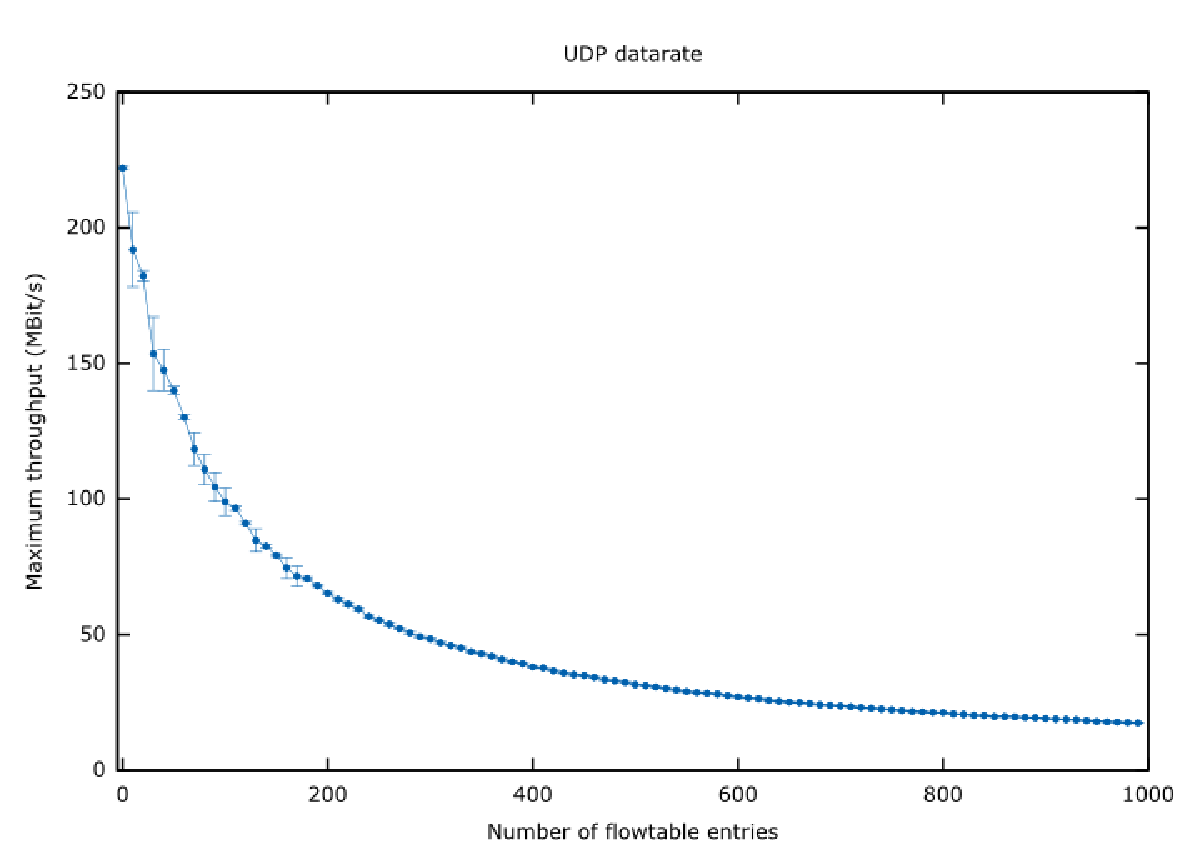
\includegraphics[height=0.7\textheight]{img/test_initial_long.eps}
\end{center}
\end{frame}

\begin{frame}
\begin{itemize}
    \item Ziel: besser werden, mehr Pakete pro Zeit durch die Matching-Einheit bekommen
    \item Idee: Umsetzung des Bitvektor-Algorithmus getrennt für alle geforderten Headerfelder
    \item Ver-UND-ung der Ergebnisse liefert dann den besten Match
\end{itemize}
Daher Austausch der bisherigen Matching-Engine in OpenFlow.
\end{frame}

\begin{frame}
\frametitle{Der Bitvektor-Algorithmus}
%%TODO: Complexity
Demo am Whiteboard
\end{frame}

\begin{frame}
\frametitle{Der Bitvektor-Algorithmus}
Komplexität: Seien $N$ Anzahl der Regeln, $k$ Anzahl der Header-Felder.\\
Dann ist Matching mit der linearen Liste in $\mathcal O(n \cdot k)$.\\
Der Bitvektor-Ansatz schafft dagegen  $\mathcal O(log\ n \cdot k)$.
\end{frame}

\section{Aktueller Stand}
\begin{frame}
\begin{itemize}
    \item Bitvektor-Implementierung in C fast fertig
    \item Integration in OpenFlow momentaner Schwerpunkt 
    \item Dabei übliche Herausforderungen (wenig Dokumentation, teilweise unübersichtliche Struktur der gegebenen Implementierung)
\end{itemize}
\end{frame}

\section{Ausblick in die Zukunft}
\begin{frame}
\begin{itemize}
    \item Testen der neuen Komponente
    \item Zusätzliche Performance durch Just-In-Time-Optimierung von häufig gerufenen Subroutinen
    \item Ausführliche Analyse und Evaluation der neuen Implementierung
\end{itemize}
\end{frame}

\section*{Fragen?}
\begin{frame}
\begin{center}
\huge{!}
\end{center}
\end{frame}
\end{document}


